\documentclass[a4paper,12pt]{article}

\usepackage[slovak]{babel}
\usepackage[left=1.5cm,text={18cm, 25cm},top=2cm]{geometry}
\usepackage[utf8]{inputenc}
\usepackage{times}
\usepackage{hyperref}
\usepackage{amsthm}
\usepackage{amsmath,amsfonts,amssymb}
\usepackage{graphicx}
\usepackage{rotating}
\usepackage{listings}
\usepackage{xcolor}
\usepackage{microtype}
\usepackage{textcomp}
\usepackage{caption}
\usepackage{relsize}
%\usepackage{subcaption}
\usepackage{subfig}
\usepackage{placeins}

\definecolor{codegreen}{rgb}{0,0.6,0}
\definecolor{codegray}{rgb}{0.5,0.5,0.5}
\definecolor{codepurple}{rgb}{0.58,0,0.82}
\definecolor{backcolour}{rgb}{0.95,0.95,0.92}

\lstdefinestyle{mystyle}{
    backgroundcolor=\color{backcolour},   
    commentstyle=\color{codegreen},
    keywordstyle=\color{magenta},
    numberstyle=\tiny\color{codegray},
    stringstyle=\color{codepurple},
    basicstyle=\ttfamily\footnotesize,
    breakatwhitespace=false,         
    breaklines=true,                 
    captionpos=b,                    
    keepspaces=true,                 
    numbers=left,                    
    numbersep=5pt,                  
    showspaces=false,                
    showstringspaces=false,
    showtabs=false,                  
    tabsize=2,
    extendedchars=false,
    escapeinside={\%*}{*)},
    inputencoding=utf8
}
\lstset{style=mystyle}

\author{Jakub Mĺkvy (xmlkvy00)}
\date{\today}
\title{\Large\bf Projekt -- IMS 2020/2021}

\begin{document}
\begin{titlepage}
	\begin{center}
	    \vspace*{+3cm}
		\Huge
		\textsc{Fakulta informačních technologií\\
		\huge Vysoké učení technické v~Brně}\\
		\vspace{\stretch{0.382}}    
	    {\LARGE{Dokumentácia\\Projekt č. 16 do predmetu:\\ \textit{Mikroprocesorové a vestavěné systémy}\\
		 \vspace{4mm}
		 \Huge\textbf{{ARM-FITkit3: \\ Měření srdečního tepu}}\\
		 \vspace{4mm}
		 2020/2021
		 }}
		 
		\vspace{\stretch{0.618}}
	\end{center}
	{\Large Jakub Mĺkvy (xmlkvy00) \hfill
	\today}
	
	\thispagestyle{empty}
    \setcounter{page}{0}
\end{titlepage}

\newpage

\tableofcontents

\newpage
\section{Úvod}

\quad Cielom projektu bolo získať pulz z prstu pomocou infračervenej diody a infračerveného snímača. Pri tlkote srdca sa tlak v tele zvyšuje každým stiahnutím. Zvýšenie tlaku teda znamená vháňanie krvi do ciev. Pri presvitaní prstu infračerveným svetlom to znamená zmena disperzie infračerveného svetla pri zmene tlaku a tým pádom aj zmena zachyteného infračerveného svetla na snímači úmerná ku zmene tlaku.

\section{Rozbor tématu a použitých technológií}

\subsection{Hardware a komponenty}
\begin{itemize}
    \item procesor MK60DN512VMD10 v ARM-FITkit3
    \item displej typu LFD039AUE-102A
    \item IR dioda
    \item IR senzor
    \item MCU
    \item LPTMR
    \item ADC
\end{itemize}
Zapojenie podľa zadania projektu. \cite{projekt}

\subsection{Prostredie}
Kinetis Design Studio 3.0 pre čip MK60D10. Implementácia v jazyku C.

\subsection{Spracovanie signálu}
Bola požitá jednoduchá forma low pass\cite{high} a high pass\cite{low} filtru a následné spriemerovania 32 samplov pre vyhladenie a normalizáciu signálu.

\section{Video}
Video pre odprezentovanie funkčnosti:\\
\href{https://drive.google.com/file/d/108AYM786Ci\_kplIACoSMAsEM9yC37Z1F/view\?usp\=drivesdk}{https://drive.google.com/file/d/108AYM786Ci\_kplIACoSMAsEM9yC37Z1F/view?usp=drivesdk}

\section{Pozorovanie}
Podarilo sa dosiahnuť správneho merania po 10 sekundách snímania pulzu s rozdielmi opakovaných meraní +-4 bpm pri úplnom klude. Hlavný nedostatok je nestabilný senzor, kde keď ruka nie je v klude môže vytvoriť dostatočne veľkú odchýlku, ktorá sa dá pomýliť za pulz.

\begin{figure}[htp]
    \centering
    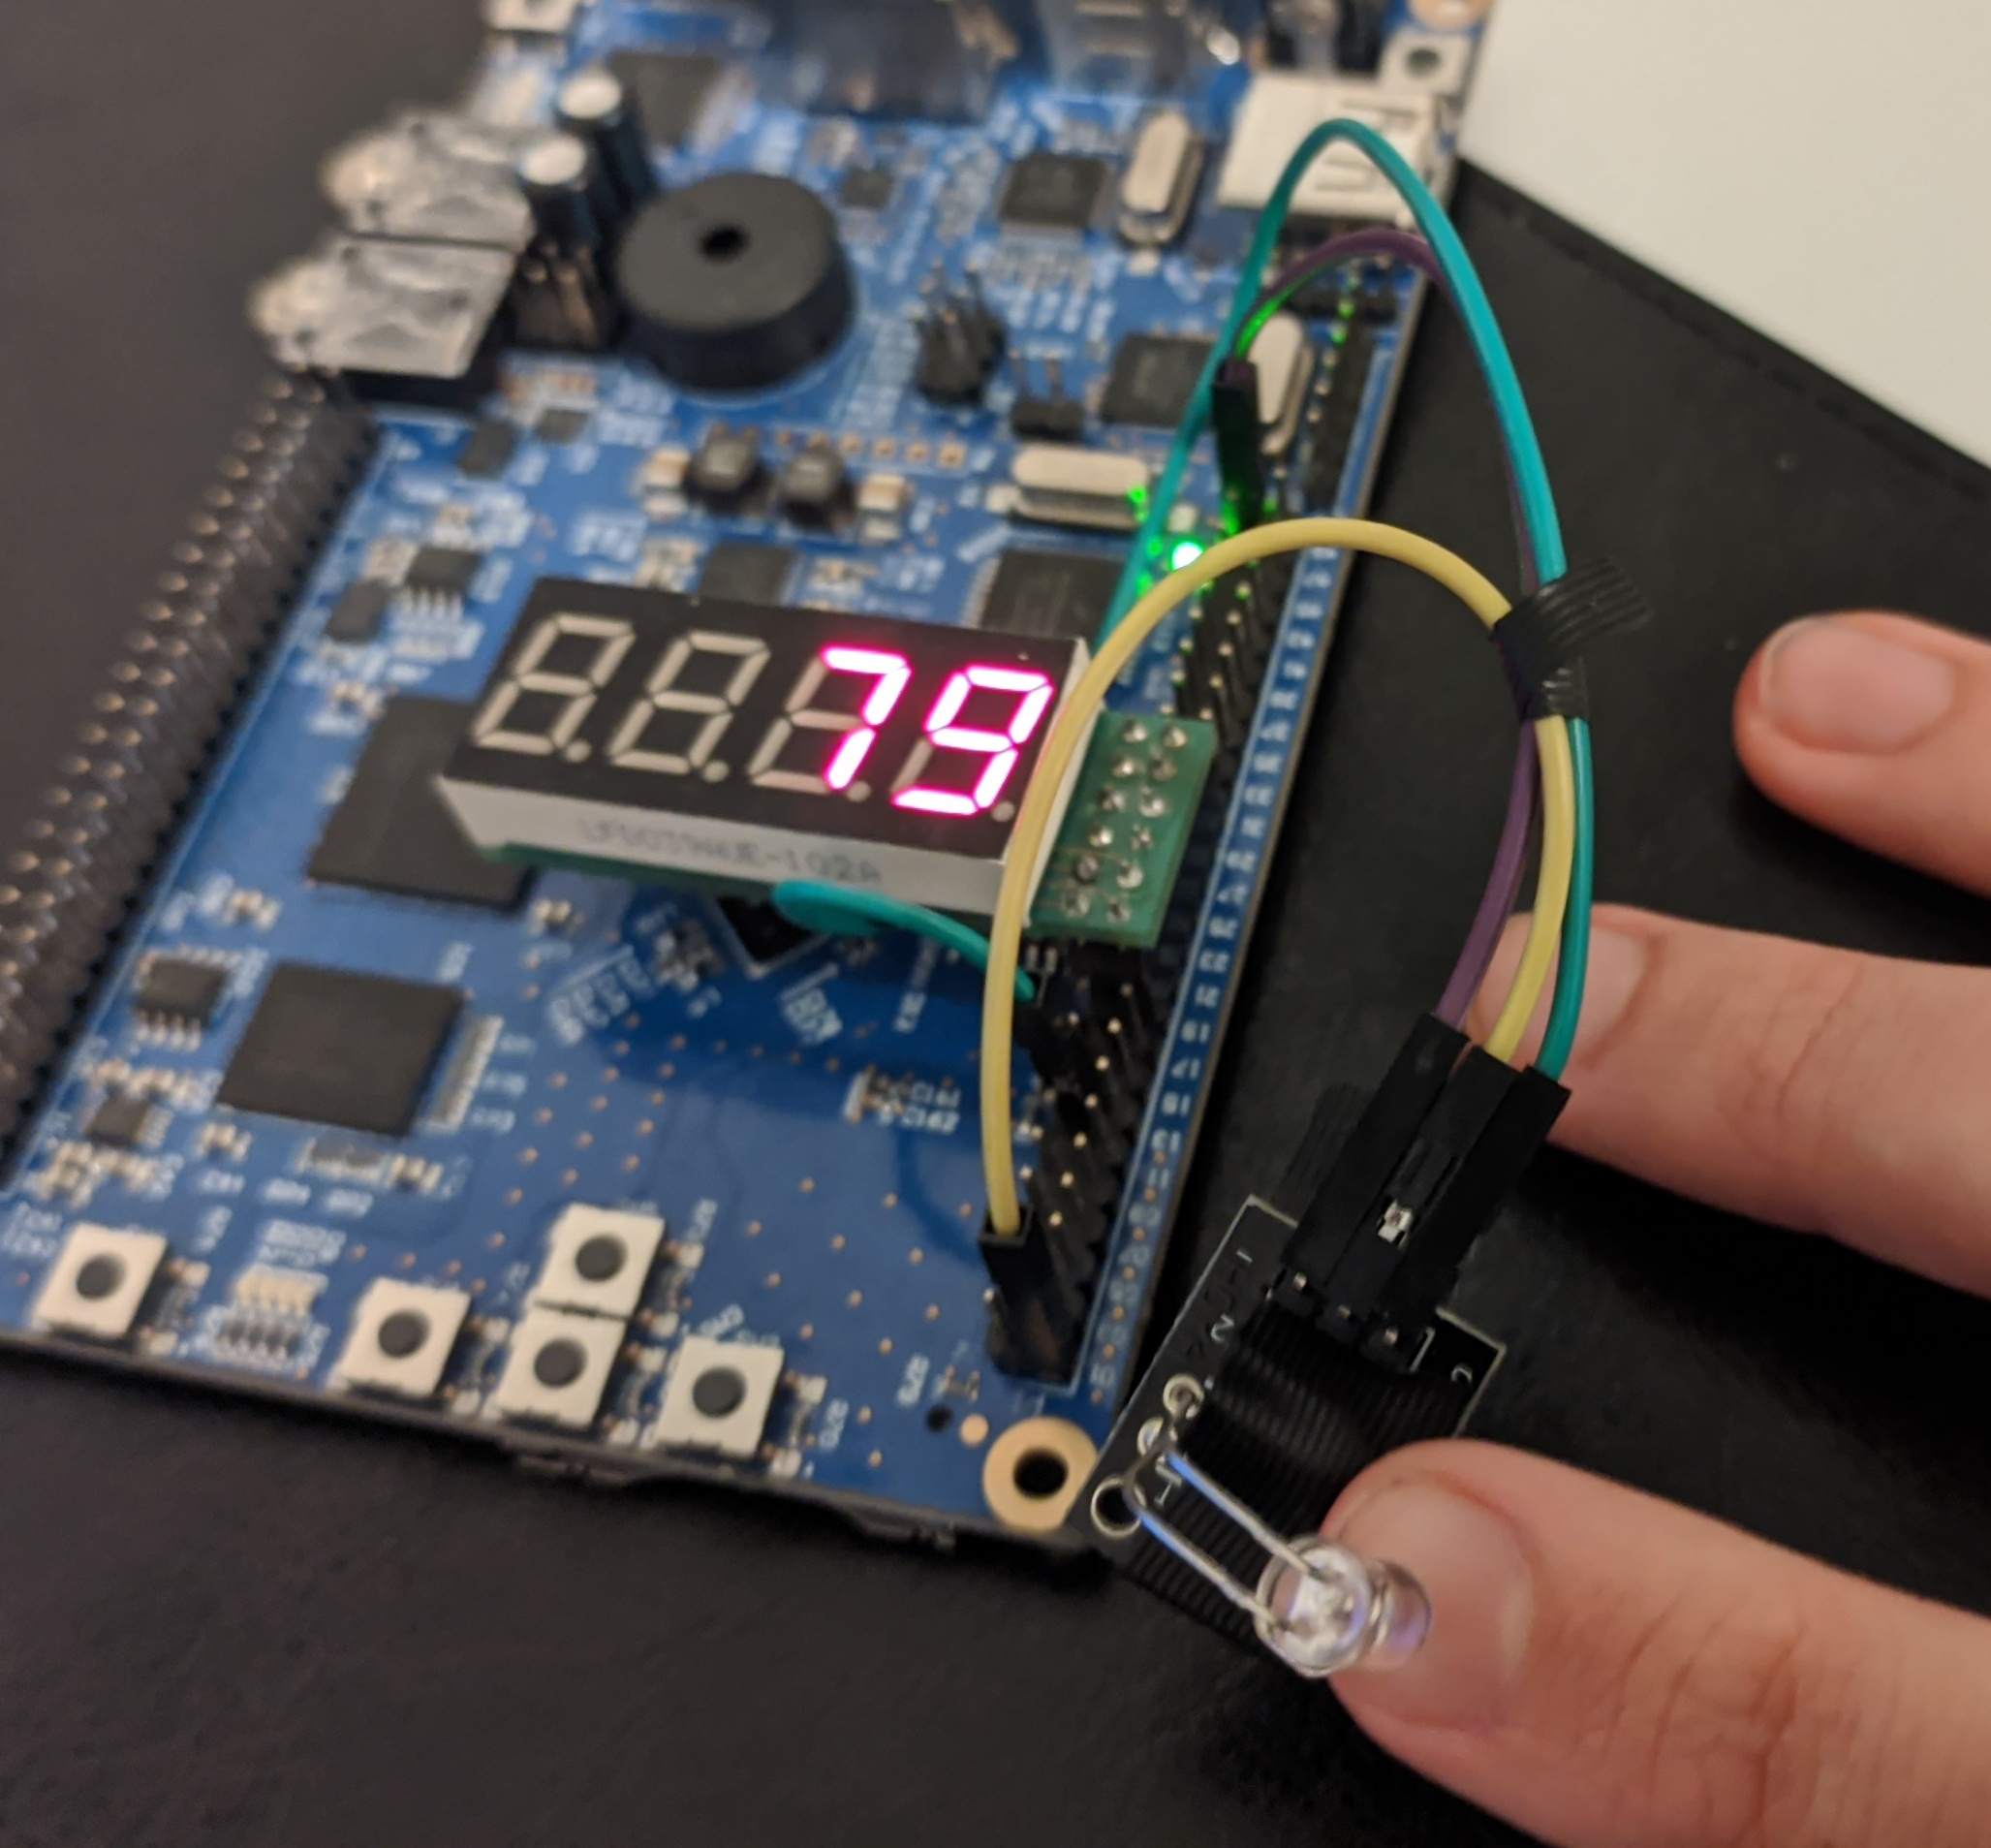
\includegraphics[width=8cm]{img1.jpeg}
    \captionsetup{justification=centering,margin=2cm}
    \label{fig:neighbor_radius}
\end{figure}

\begin{figure}[htp]
    \centering
    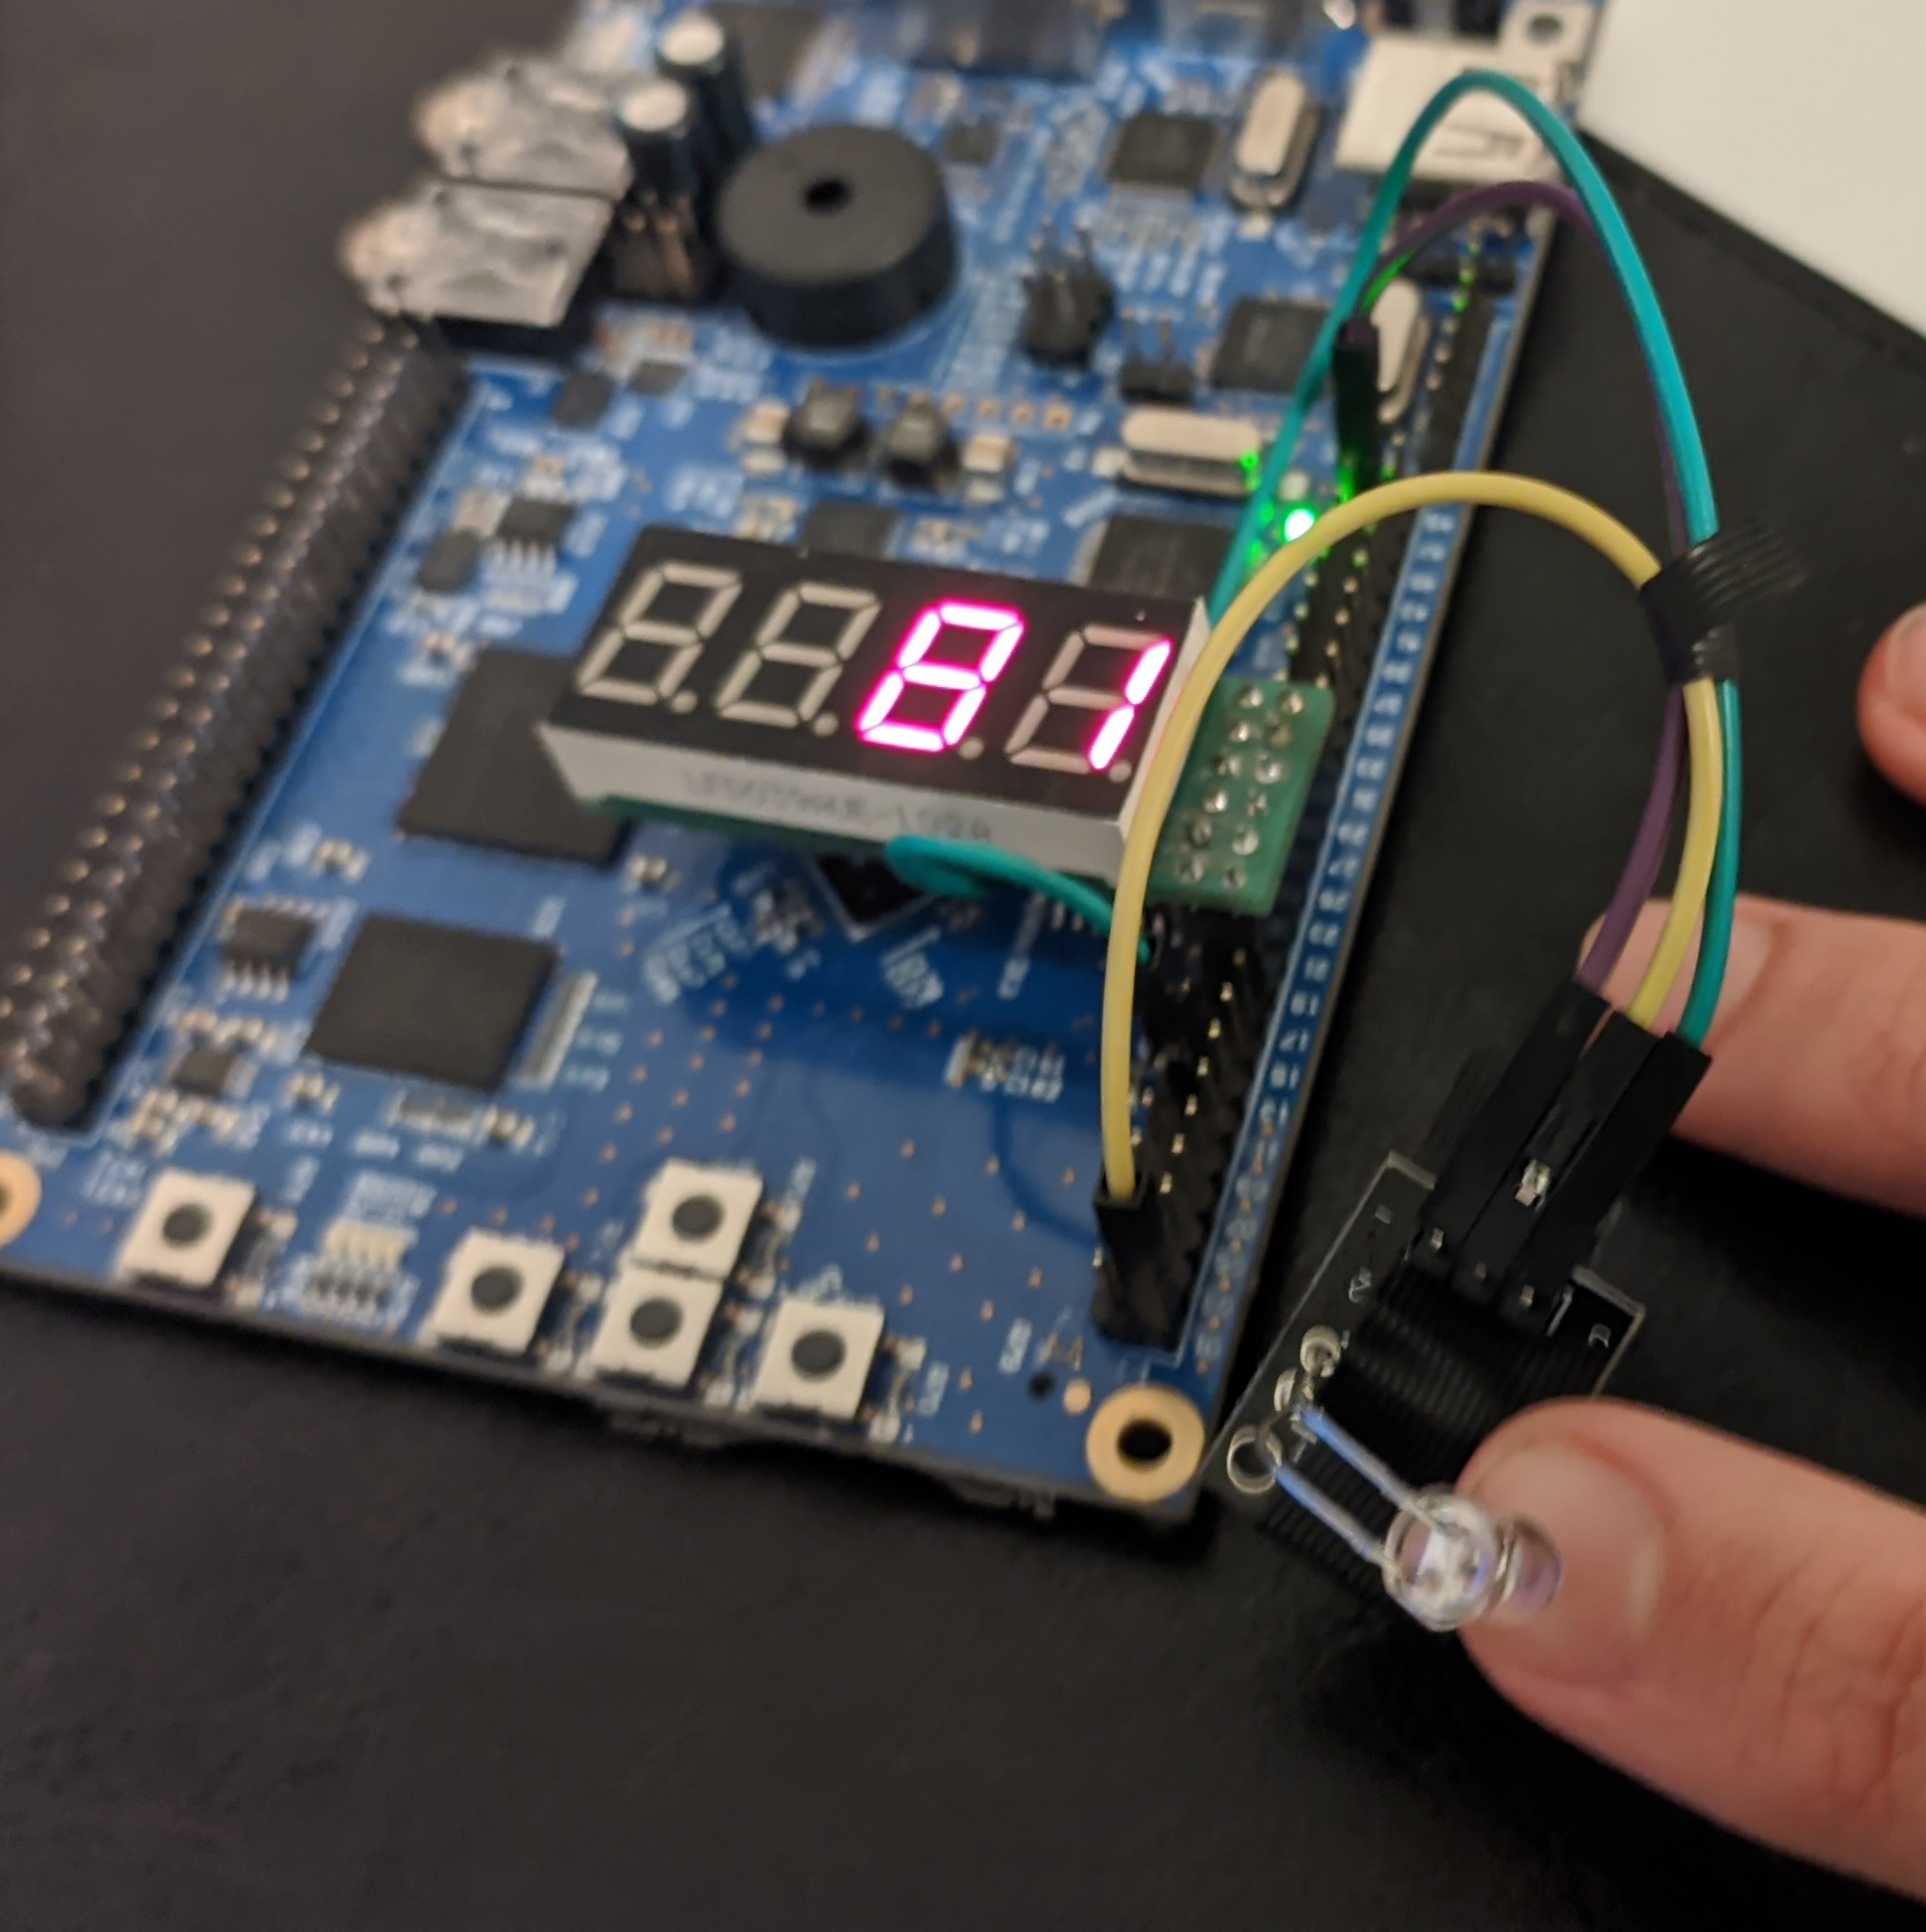
\includegraphics[width=8cm]{img2.jpeg}
    \captionsetup{justification=centering,margin=2cm}
    \label{fig:neighbor_radius}
\end{figure}

\begin{figure}[htp]
    \centering
    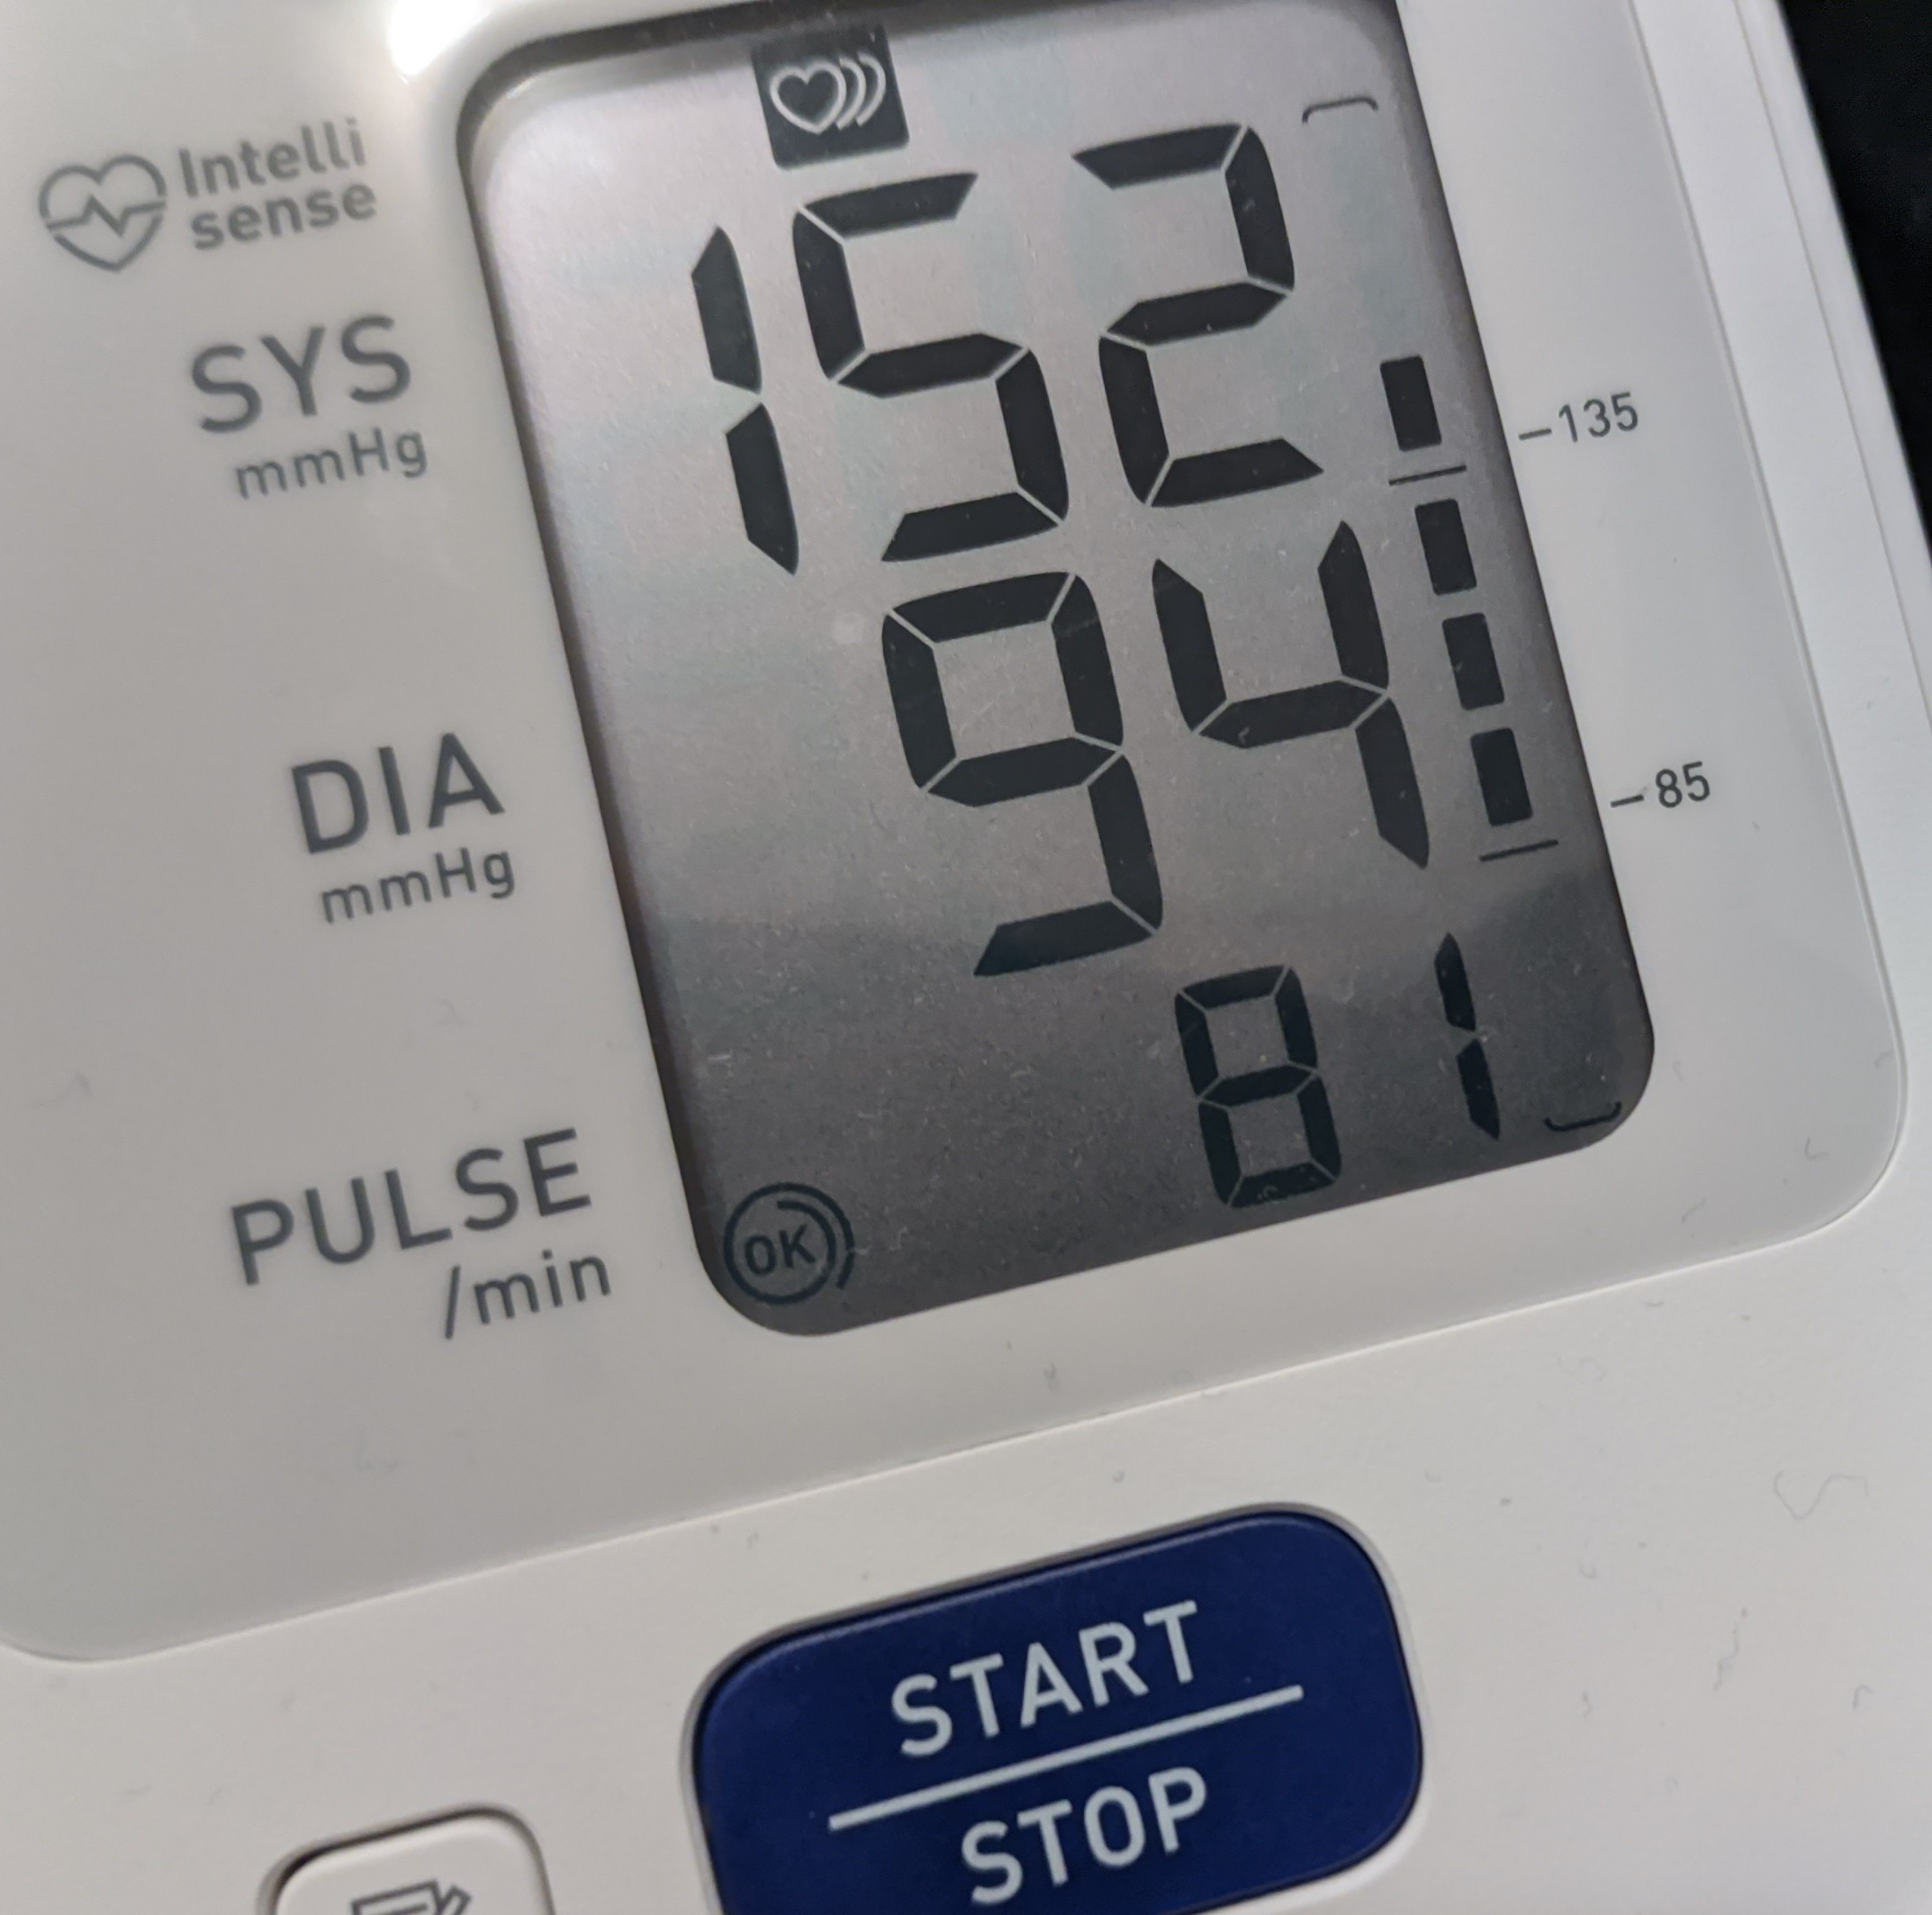
\includegraphics[width=8cm]{img3.jpeg}
    \captionsetup{justification=centering,margin=2cm}
    \label{fig:neighbor_radius}
\end{figure}

\newpage
\section{Bibliografia}
\bibliographystyle{czechiso}
\bibliography{manual}
\nocite{projekt}
\nocite{high}
\nocite{low}
\nocite{fireSpread}
\nocite{konceptModel}

\end{document}